\chapter{Generalist Robots and the Data Bottleneck}
\minitoc
This Chapter descripes the overall goal of Robotics, to develop an generalist robot that can perform a wide variety of tasks in unstructured, unseen real-world environments. It also introduces to the data bottleneck in robotics, which arises from the limited availability of large, diverse, and high-quality datasets and hinders the development of an generalist robot. The chapter discusses different data sources for robot learning, including real-world robot data, simulated data, and internet data, and highlights the challenges and opportunities associated with each source. Finally, it emphasizes the importance of leveraging large-scale internet video data to address the data bottleneck and improve robotic learning capabilities.
% Classical robotics techniques are insufficient as they cannot handle unseen and unstructured scenarios \cite{Krotkov_DARPA_2017}.


\section{Generalist Robots}
The ultimate goal of robotics is to develop a \textbf{generalist robot}. According to McCarthy et al. \cite{McCarthy_2025}, such a robot should be able to perform a wide variety of physical tasks in unstructured, unseen real-world environments. It must combine high-level reasoning and planning abilities with low-level physical skills, such as dexterous manipulation. Furthermore, it should be capable of adapting to unforeseen situations and operate under imperfect and partial observations, for example through visual and tactile sensing. In summary, a general-purpose robot is capable of adapting to different situations and learning new skills just like humans \cite{tsujiSurveyImitationLearning2026}. Such a robot would be highly useful across a wide range of real-world applications. 

\paragraph{Application Field: Industrial Settings}
In industrial settings, this would enable robots to be deployed flexibly across different environments and tasks, without the need for task-specific or environment-specific programming or retraining. As a result, robots could also be utilized for spontaneous small, short-term tasks, where automation is currently not economically viable due to high setup costs and effort. This increased flexibility would lead to higher utilization rates and, consequently, reduced long-term operational costs \cite{tsujiSurveyImitationLearning2026}.

\paragraph{Application Field: Household Settings}
In addition, general-purpose robots could play an important role in household settings. They could assist with everyday tasks such as tidy up rooms, loading/unloading dishwashers, setting tables, or acting as general assistants for example helping to carry objects.

\paragraph{Application Field: Healthcare and Assistive Settings}
In healthcare and assistive contexts, such robots could support individuals with limited mobility by helping them perform daily activities, such as standing up, sitting down, opening a door, or transporting objects. This highlights the potential of generalizing robotic systems to improve both efficiency in industry and quality of life in everyday and care settings \cite{tsujiSurveyImitationLearning2026}.

\subsection{Ethical Concerns} 
Ethical concerns regarding the development of generalist robots should not be underestimated and must not be ignored. In the future, robots are likely to take over many tasks, particularly those that are repetitive and monotonous, which may lead to the displacement of certain jobs. Whether this could result in large-scale unemployment due to automation remains a subject of ongoing debate.

Furthermore, once the technology has sufficiently matured, such robots could also be used for \texttt{military purposes}. While this could reduce the risks to human soldiers, it also raises serious ethical concerns, as it makes forms of automated or autonomous warfare increasingly conceivable.

It is therefore essential that the development and deployment of generalist robots are carried out responsibly and in accordance with ethical guidelines, in order to minimize potential negative impacts on society.


\section{Data Bottleneck in Robotics}
A central question in robotics is how to train a generalist robot capable of performing a wide range of tasks in unstructured and previously unseen real-world environments?

\textit{Usage of Large-Scale Datasets.} Progress in related machine learning domains—such as Natural Language Processing \cite{Achiam2023GPT4TR}, Computer Vision \cite{betkerImprovingImageGeneration}, and video generation \cite{videoworldsimulators2024}—suggests that large-scale datasets and model capacity are key drivers of performance and generalization capabilities. 
Training high-capacity models with expressive architectures on diverse, extensive internet-scale datasets has led to the emergence of robust representations and improved out-of-distribution performance in these domains \cite{Vaswani2017AttentionIA}.
Empirically, these improvements often follow predictable scaling laws, where performance improves as more data, model size, and compute are used \cite{kaplan2020scalinglawsneurallanguage}.
Recent work suggests that similar scaling behavior may also apply to robotics and \ac{IL}. For example, studies show that robots generalize better when they are trained on more diverse training data, including variations in environments, objects, and tasks \cite{lin2024data,open_x_embodiment_rt_x_2023}. Large-scale \ac{IL} approaches based on \ac{BC} have demonstrated that training a single policy across many tasks yields substantial gains in robustness and generalization. For example, transformer-based robot policies such as RT-1 and RT-2 leverage large, heterogeneous datasets to achieve zero-shot generalization to novel tasks and instructions \cite{rt12022arxiv, rt22023arxiv}.
% Moreover, approaches such as large-scale behavioral cloning across multiple tasks have shown promising zero-shot generalization capabilities in novel settings \cite{rt12022arxiv}.
% Approaches based on large-scale behavior cloning across multiple tasks have also demonstrated promising results, including zero-shot generalization to new settings. 

\textit{Data bottleneck.} In contrast to vision and language domains, robotics is fundamentally constrained by the cost and complexity of data collection, limiting the availability of large, diverse, and high-quality datasets. High-quality demonstrations require physical real world interaction, making them time-consuming to acquire, and are often limited in diversity due to hardware and safety constraints \cite{tsujiSurveyImitationLearning2026}.
As a result, available datasets are usually smaller and less diverse. Consequently, this data scarcity represents a major bottleneck for achieving similar levels of scalability and generalization in robot learning, and remains a central challenge in the development of general-purpose robotic systems \cite{tsujiSurveyImitationLearning2026}.


% In contrast to vision or language domains, robotics faces a fundamental limitation: the lack of large, diverse, and high-quality datasets.
% \subsection{Relevant Data Categories for Robotics}
\subsection{How to Address the Data Bottleneck}
How can we address this data bottleneck in robotics? Before discussing specific approaches, it is important to clarify which data sources are relevant for robot learning and how such data can be acquired.

\paragraph{Real World Robot Data}

	% A high quality data source is real world data, which can be collected directly from the robot's interactions with the environment.
	Real-world robot data is obtained through physical interaction between the robot and its environment and represents a high-quality source for robot learning. Through direct interaction, trajectories and sensor measurements can be recorded under real operating conditions, capturing effects such as sensor noise and environment variability that are difficult to model accurately in simulation.

	\textit{Data Collection via Teleoperation.} A common approach to collecting such data is human teleoperation, where an operator controls the robot to perform tasks and generate demonstration trajectories \cite{Bousmalis2023RoboCatAS, Khazatsky2024DROIDAL, OpenXR}. This type of data has been widely used in \ac{IL} and has contributed to the development of early robot foundation models \cite{Bousmalis2023RoboCatAS, Team2024OctoAO}. 
	Teleoperation can be realized through various control interfaces, including joysticks, motion-capture systems, or virtual reality setups. 
	Teleoperation enables precise control and is particularly suitable for collecting demonstrations of complex manipulation tasks that require fine-grained movements and accurate timing. However, it is time-consuming and often requires specialized hardware, which limits scalability. To mitigate this, datasets are increasingly aggregated across multiple research institutions, improving both scale and diversity \cite{OpenXR}.

	% recent work has explored methods for automating the data acquisition process. These approaches aim to reduce human involvement by enabling robots to collect data autonomously or semi-autonomously.
	\textit{Data Collection Improvements.} To further address the limitations of manual data collection, recent work has explored automated or semi-automated data acquisition methods, where robots collect data with reduced human intervention \cite{Bousmalis2023RoboCatAS, Ahn2024AutoRTEF, Yang2023RobotFM}. In parallel, advances in robotic infrastructure, particularly in industrial settings, indicate that large-scale data collection in real-world environments is becoming increasingly feasible \cite{McCarthy_2025}.

	Despite these developments, real-world datasets remain significantly smaller and less diverse compared to internet-scale datasets used in vision and language domains. This limitation continues to pose a challenge for scaling robot learning methods and achieving robust generalization.


\paragraph{Simulated Data}
	
	\textit{Simulatedly Generated Demonstration Data.} 
	Simulation enables the generation of robot trajectories in virtual environments without the cost, safety risks, and hardware limitations associated with real-world experiments. As a result, simulated demonstrations can be used in scenarios where collecting physical robot data would be impractical, expensive, or unsafe \cite{Kaufmann2023ChampionlevelDR, Zhang2022FineGrainedEH, Nasiriany2024RoboCasaLS}.
	These generated trajectories are commonly used in \ac{IL} especially in Behavior Cloning, where policies are trained on demonstration.

	Expert demonstrations in simulation are typically generated by executing a high-performing controller or policy in the simulated environment. This can be a hand-crafted controller, a planning-based system, or a policy obtained via \ac{RL}.
	\begin{itemize}
		\item \textbf{Hand-Crafted Controllers:} 
		Hand-crafted controllers are based on classical control methods such as PD/PID controllers, Linear Quadratic Regulators, or Model Predictive Control \cite{PredictiveControlTwoWheeled, ModelPredictiveControl2022}. These methods are particularly effective for low-dimensional tasks, including balancing, set-point tracking, or waypoint following, where they can generate stable and accurate trajectories. However, they often struggle in complex or high-dimensional environments.
		\item \textbf{Rule-Based and Planning-Based Systems:} 
		For manipulation and navigation tasks, motion planning algorithms such as A*, PRM, or RRT* can be used to compute collision-free trajectories. Frameworks such as MoveIt \cite{MoveIt2Documentation} integrate these planning methods with low-level robot controllers and are widely used in robotics applications \cite{DBLP_journals_corr_abs_2103_12826}. These approaches can generate high-quality demonstrations but often require accurate environment models and can become computationally expensive in complex scenarios.

		\item \textbf{Policies Obtained via Reinforcement Learning:}
		Another approach is to train a \ac{RL} policy, froze it and use it to generate expert demonstration trajectories for downstream \ac{IL} \cite{ParkerHolder2022EvolvingCW, Liang2024EurekaverseEC}. Compared to hand-crafted or planning-based approaches, \ac{RL} policies can better adapt to high-dimensional and complex tasks, although training them typically requires large amounts of interaction data and computational resources \cite{McCarthy_2025}.

		In simulation, these policies can additionally be trained using \textit{privileged simulation information}, which would not be accessible in real-world settings \cite{Ha2023ScalingUA, Geng2023UniDexGraspID, Dalal2023ImitatingTA}. Examples include exact object positions, velocities, segmentation masks, or the full environment state. Access to this additional information can simplify the learning process and improve the quality of the generated trajectories.

		Another opportunity is to simplify the problem by training separate expert policies for each subtask. For example, train one policy for grasping, one for navigation, and one for the pulling motion for opening drawers and coordinate them to form a complete task.
		
		
	\end{itemize}

	\textit{Online Learning in Simulation.} 
	% 	Simulation also allows for online learning, where the robot can interact with the simulated environment and collect new data during training. This is particularly beneficial for reinforcement learning, which typically requires extensive interaction with the environment to learn effective policies. By leveraging simulation, we can significantly accelerate the learning process and enable safe exploration of a wide range of scenarios.
	In addition to generating demonstration datasets, simulation is widely used for online learning in robotics, particularly in \ac{RL}. In online learning, the robot continuously interacts with the environment and improves its policy based on newly collected experience during training. Simulation is especially suitable for this process because it enables safe exploration and automatic resetting of environments, parallelized data collection, and faster-than-real-time execution without risking damage to physical hardware. Consequently, simulation has become an essential component for scalable robot learning systems that require large amounts of interaction data, particularly in RL \cite{Zhuang2023RobotPL, Kaufmann2023ChampionlevelDR, Nasiriany2024RoboCasaLS}.
	
	\textit{Sim-to-Real Gap.} 
	Despite its advantages, simulation-based robot learning faces several important challenges \cite{Bharadhwaj2024PositionSS}. One major issue is the sim-to-real gap, which arises from inaccuracies between simulated and real-world physics. Effects such as friction, contact dynamics, deformable objects, latency, and sensor noise are often difficult to model accurately. This gap can lead to poor performance when transferring policies trained in simulation to real robots \cite{DBLP:journals/corr/abs-2009-13303}.
	% , causing policies trained in simulation to generalize poorly when transferred to physical robots. 
	A common strategy to mitigate this problem is domain randomization, 
	% where various parameters of the simulation
	where environmental properties such as textures, lighting conditions, physical parameters, and sensor characteristics 
	are randomized during training to improve robustness and transferability \cite{Tobin2017DomainRF}.

	\textit{Task Diversity.}
	Another limitation is the difficulty of creating sufficiently diverse simulated tasks and environments for general-purpose robot learning. Manually designing large numbers of environments is labor-intensive and does not scale efficiently. Recent work therefore explores procedural environment generation, where environments and task configurations are generated automatically to increase diversity and improve policy generalization \cite{Deitke2022ProcTHORLE, Team2023HumanTimescaleAI, Xian2023TowardsGR, Faldor2024OMNIEPICOV, Wang2023RoboGenTU}. 

	Despite these challenges, simulated demonstrations remain a valuable source of training data for \ac{IL}, as they enable scalable trajectory generation and rapid experimentation in controlled environments.



\paragraph{Internet Data.}
	Internet data is a promising source for robot learning and includes various types of freely available data, such as text, images, videos, and structured information. Its main advantage lies in its scale and diversity, which can improve the robustness, adaptability, and generalization capabilities of learned robot policies \cite{McCarthy_2025,Eze2024LearningBW}. In analogy to recent advances in natural language processing and computer vision, robotics can similarly benefit from leveraging vast, weakly labeled data from the web. 
	
	In particular, these data sources can support robot learning in several complementary ways. For example, image and video datasets have been used to pretrain vision models that provide robust visual representations for robotic perception systems \cite{Nair2022R3MAU, Wang2022VRL3AD}. In addition, \acp{VLM} and \acp{LLM} have been employed to define reward functions and task objectives for robot learning \cite{Tam2022SemanticEF, Du2023VisionLanguageMA, Yu2023LanguageTR, Klissarov2023MotifIM}. \acp{LLM} have also been used as high-level planners for long-horizon tasks by decomposing complex goals into smaller executable actions \cite{Ahn2022DoAI, Huang2022InnerME}. Furthermore, several recent works adapt internet-pretrained foundation models for robotics through fine-tuning on robot-specific datasets \cite{Brohan2023RT2VM, Kim2024OpenVLAAO}, while others jointly train on both internet data and action-labeled robot trajectories to improve generalization and cross-domain transfer capabilities \cite{Reed2022AGA}.
	
	In this work, the focus lies on internet video data, which is discussed in more detail in the following sections.



\paragraph{Combination of Data Sources.} 
In modern robot learning systems, simulation data, real-world data, and internet data are rarely used in isolation. Instead, these data sources are commonly combined, as each category provides complementary strengths and addresses different limitations. 
Simulation enables scalable and cost-efficient data generation and provides a safe environment for online robot interaction and \ac{RL} \cite{DBLP_journals_corr_abs_1710_06537, DBLP:journals/corr/abs-2009-13303, DBLP_journals_corr_abs_1710_06537, DBLP:journals/corr/abs-2111-00956}. Internet data offers large-scale and diverse semantic information \cite{open_x_embodiment_rt_x_2023, rt22023arxiv}, while real-world data captures accurate physical interactions, sensor characteristics, and real-world dynamics that are difficult to model in simulation \cite{DBLP:journals/corr/abs-2111-00956}.

Typical robot learning pipelines therefore combine these data sources hierarchically \cite{rt22023arxiv, nvidia2025gr00tn1openfoundation}. In many approaches, perception and policy models are first pretrained on large-scale simulation and/or internet datasets in order to learn robust and generalizable representations. Subsequently, the models are fine-tuned on smaller but high-quality real-world robot datasets to adapt them to specific robotic platforms, sensors, and target environments \cite{open_x_embodiment_rt_x_2023}. Some works additionally employ hybrid training strategies that combine simulated and real-world data using techniques such as domain randomization or domain adaptation to further reduce the gap between simulated and real-world observations \cite{Tobin2017DomainRF, DBLP:journals/corr/abs-1812-07252}.




\subsection{Reduce the Amount of Robot Data}
To train a generalist robot, large amounts of diverse data are required in order to capture the variability of real-world environments and tasks \cite{McCarthy_2025, Eze2024LearningBW, Kawaharazuka2025VisionLanguageActionMF, Din2025VisionLA}. In particular, robot interaction data, also known as robot data, is highly valuable because it contains both observations of the environment, such from RGB-D cameras or other sensors, and the corresponding robot trajectories and actions. This enables the robot to learn the relationship between observations, actions, and their resulting outcomes.

However, the currently available amount of robot data is still insufficient in both scale and diversity to train highly generalizable robotic systems \cite{McCarthy_2025}. Collecting robot data, whether in real-world environments or in simulation, is expensive and time-consuming. Real-world data collection requires physical hardware, human supervision, and extensive interaction time, while simulation environments often suffer from the sim-to-real gap and still require significant engineering effort \cite{McCarthy_2025}. As a result, data scarcity remains one of the central challenges in the development of general-purpose robotic systems.


\textbf{Large-Scale Internet Video Data.} To address this data bottleneck, one promising approach is to leverage large-scale internet video data \cite{McCarthy_2025}. Internet videos provide a rich source of information about human behaviors, object interactions, and task execution in diverse environments that are relevant for robotics. They contain fundamental information about physical dynamics, a wide variety of scenarios and interactions (motion patterns), and semantic task structure that can be useful for robotic learning. In contrast to robot datasets, internet-scale video data is abundant, inexpensive to obtain, and covers a much broader range of scenarios and activities as robot datasets \cite{McCarthy_2025}. 
% By augmenting traditional robot data with large-scale internet video, we can significantly enhance the learning capabilities of robotic systems and enable them to perform effectively in real-world settings \cite{lin2024data}.

Although such videos typically do not contain direct robot actions, recent work has shown that they can still provide strong supervisory signals for representation learning, action understanding, and policy pretraining. By augmenting traditional robot datasets with large-scale video data, robotic systems can learn more robust and transferable representations, improving their ability to generalize to unseen tasks and environments \cite{lin2024data}.


\paragraph{Formalism.} 
According to \cite{McCarthy_2025}, the data is formalized as follows:
\begin{itemize}
	\item $D$: The complete training dataset used for learning the robotic policy.
	% The full Dataset which is available for training the robot model.
	This dataset is a combination of the categories real-world data, simulated data, and internet data. $D$ can be subdivided into two subsets: $D = \{D_{robot}, D_{video}\}$. 
	
	\item $D_{robot}$: Subset of dataset $D$ containing robot interaction data collected from physical robots in real-world or simulation environments, including observations and the robots corresponding actions obtained during interaction. Each sample in $D_{robot}$ consists of transition tuples of the form $(o_t, a_t, r_t, o_{t+1})$, where $o_t$ is the observation at time $t$, $a_t$ is the action taken by the robot, $r_t$ is the reward received after taking action $a_t$, and $o_{t+1}$ is the resulting observation after executing action $a_t$. The reward $r_t$ may be missing, and each $o$ contains an image observation and can additionally contain other information, such as depth or tactile data. 
	
	% \item $D_{robot}$: Subset of dataset $D$ that consists of real-world or simulated robot data, which includes observations and corresponding actions collected from physical interactions. Technisch gesehen, beinhaltet D_{robot} transition tuples of $(o_t, a_t, r_t, o_{t+1})$, where $o_t$ is the observation at time $t$, $a_t$ is the action taken by the robot, $r_t$ is the reward received after taking action $a_t$, and $o_{t+1}$ is the resulting observation after executing action $a_t$. The reward $r_t$ may be missing, and each $o$ contains an image observation and can additionally contain other information, such as depth or tactile data. 
	% This data is crucial for learning the relationship between actions and their outcomes in real-world settings.
	\item $D_{video}$: Subset of the dataset $D$ that consists the video (demonstration) data. $D_{video}$ can be obtained from external sources such as internet videos. A video clip is represented as $\tau=(o_0, o_1, ..., o_T)$, where $\tau$ denotes the full video clip and each observation $o_t$ corresponds to an RGB image. Depending on the dataset, videos may additionally be paired with language descriptions, action annotations, or other auxiliary modalities.
	% $D_{video}$ may come paired with language annotations or annotations of other modalities.

\end{itemize}

\begin{figure}[!ht]
	\centering
	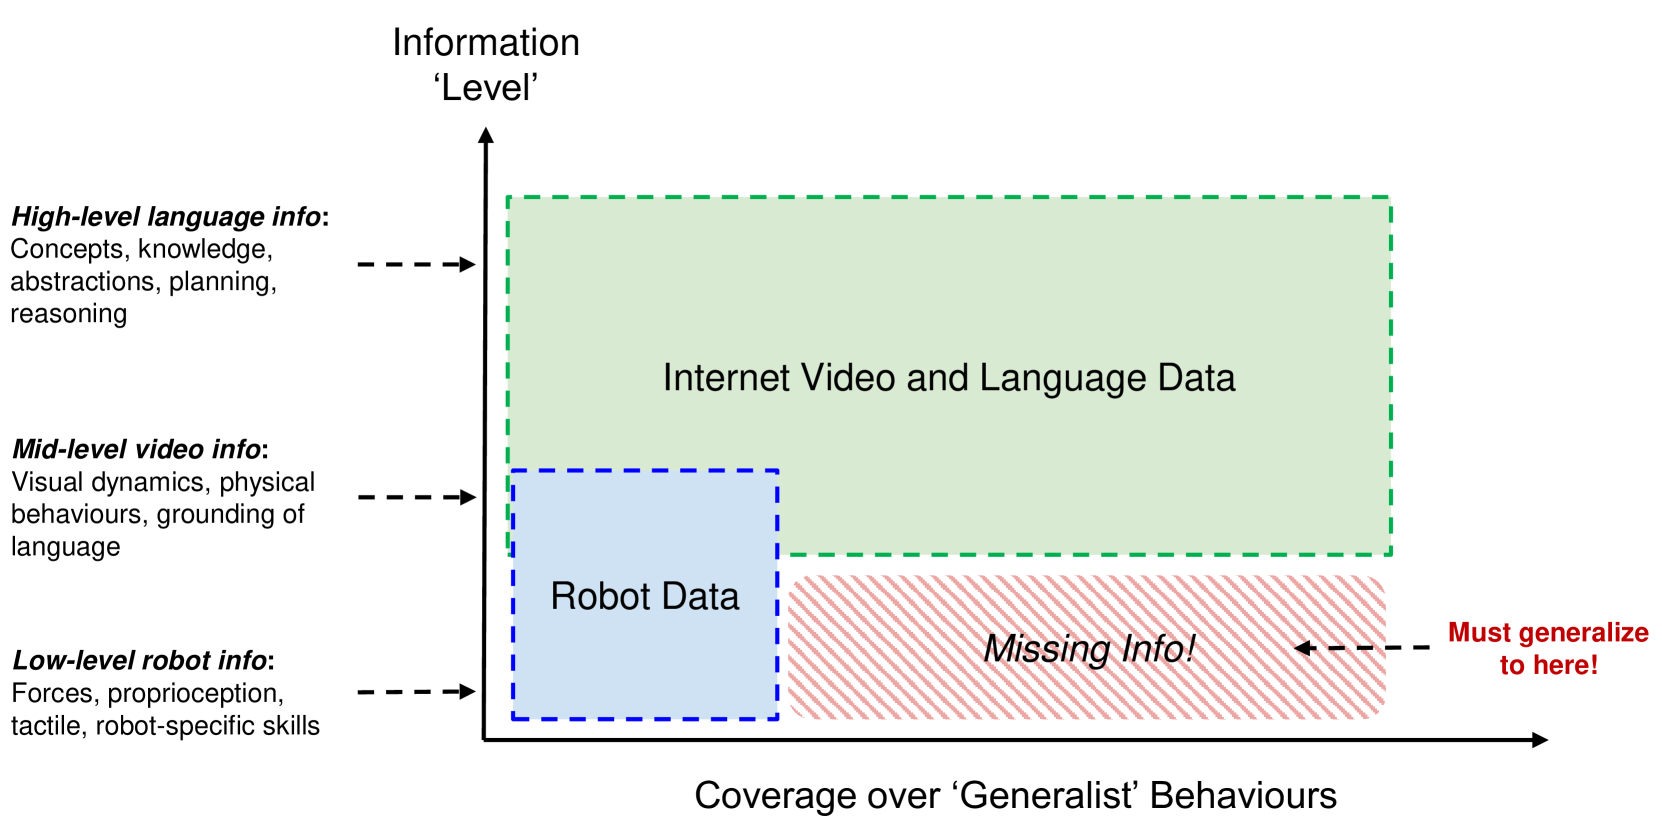
\includegraphics[width=1.0\linewidth]{./chapter4/media/DataBottleneck}
	\caption[Problem: Data Bottleneck in Robotics]{Problem: Data Bottleneck in Robotics. Image source: \cite{McCarthy_2025}.}
	\label{fig:DataBottleneck}
\end{figure}

Figure \ref{fig:DataBottleneck} illustrates the  data bottleneck in robotics. The x-axis represents the spectrum of behaviors that a generalist robot is expected to perform, while the y-axis reflects the different levels of information present in various data sources. The figure highlights that, although internet data encompasses a broader range of behaviors in diverse real-world scenarios compared to specialized robot datasets, it often lacks the detailed, low-level information that is critical for robotic applications.  
Ideally, for every relevant behavior, both low-level robot data and internet data would be available, allowing a model to establish connections across different information levels. However, as illustrated in Figure \ref{fig:DataBottleneck}, there is a significant lack of low-level robot data for many behaviors that are well represented in internet data (see ``Missing Info'' area). 
% This gap in fine-grained information presents a major challenge for learning generalist robotic skills from diverse data sources.
This absence of fine-grained information poses a significant challenge for generalizing robot learning beyond the limitations of available robot datasets \cite{McCarthy_2025}. Overcoming this gap and effectively leveraging both broad internet data and precise robot data is a central objective in advancing \ac{LfV} approaches \cite{McCarthy_2025}.



\textit{Goal of Learning from Videos.} \ac{LfV} aims to exploit this abundance of video data to improve robotic learning. \cite{McCarthy_2025} says, the goal of \ac{LfV} is to leverage our combined \ac{LfV} dataset, $D = \{D_{robot}, D_{video}\}$, to obtain an improved policy $\pi(a_t | s_t)$ versus when learning from $D_{robot}$ alone. 


% While robot datasets provide precise information about robot actions and control, video datasets contain high-level information about how tasks are performed in diverse real-world scenarios. Combining both sources of data can therefore help robotic systems learn beyond the limitations of traditional robot-only datasets.


\paragraph{Improvements of Learning from Videos.} 
What can we expect from combining both data sources, $D_{\text{robot}}$ and $D_{\text{video}}$, instead of using only $D_{\text{robot}}$? 

\begin{itemize}
	\item \texttt{Generalization beyond $D_{\text{robot}}$.}
	One important improvement of \ac{LfV} is the potential to generalize beyond the limited set of tasks contained in the robot dataset $D_{\text{robot}}$ \cite{Eze2024LearningBW}. While robot data primarily provides information about low-level robotic skills, such as grasping or locomotion \cite{Chen2024RH20TPAP}, internet-scale video data contains a much broader variety of tasks and human behaviors. By combining both data sources, models may learn how low-level robot actions relate to higher-level task structures observed in videos. As a result, an \ac{LfV} system may be capable of solving tasks that are not explicitly present in $D_{\text{robot}}$ but are represented within $D_{\text{video}}$ \cite{Brohan2023RT2VM, Du2023LearningUP, Wu2023UnleashingLV, Wang2023MimicPlayLI}.

	\item \texttt{Emergent Capabilities.}
	In natural language processing and computer vision, the availability of large-scale internet data has led to significant improvements and, in some cases, the emergence of capabilities that were not explicitly trained for \cite{Radford2019LanguageMA, Brown2020LanguageMA}. Similar progress is expected in robotics. By combining robot interaction data with internet-scale video data with language annotations, models may learn to connect low-level robotic skills with rich semantic abstractions and higher-level world knowledge obtained from textual data \cite{Achiam2023GPT4TR}. This combination has the potential to improve generalization, task understanding, and the ability to solve previously unseen tasks.

	\item \texttt{Improvements in-distribution of $D_{\text{robot}}$.}
	Furthermore, video data may also improve performance on tasks that are already represented within the robot dataset $D_{\text{robot}}$ . Since robot demonstrations are expensive to collect, additional video data can improve data efficiency and help models learn more robust visual and task representations \cite{Nair2022R3MAU}. As a result, \ac{LfV} approaches may achieve higher task success rates and overall better performance compared to approaches trained solely on robot interaction data \cite{Wu2023UnleashingLV}.
\end{itemize}










\paragraph{Information Levels:}
Robot data primarily contains low-level and mid-level information and can be collected from both real-world and simulation, with real-world data being more valuable. In contrast, internet data is typically richer in mid-level and high-level information. The following sections explain each information level in detail.

\begin{itemize}
	\item \textit{Low-Level Robot Information.} 
	Low-level robot information refers to sensory and control signals that directly describe the robot's physical state, motion, and interaction with its environment. This includes, for instance, end-effector pose, joint positions, joint velocities, joint torques, and gripper state (e.g., open or closed). Additionally, low-level information includes information about the physical forces acting on the robot itself. In simulation environments, they may include physical details of objects in the environment, such as contact forces, object properties or object dynamics.
	Such low-level informations are essential for learning precise motor control tasks, including grasping, locomotion, and manipulation.

	\textbf{Proprioceptive information} refers to the robot's internal sense of its own body and movement. It includes data about the robot's end-effector pose which implicity inlcudes joint angles, joint velocities, and gripper configuration. This information is crucial for executing accurate and stable motions, as it allows the robot to understand its current state and adjust its actions accordingly. 
	A robot may visually observe a cup through a camera and wants to grasp it. Proprioceptive information tells the controller how to move the arm to the cup, which includes:
	\begin{itemize}
		\item what is the current pose/state of the robot
		\item how far the arm has moved,
		\item whether the wrist is rotated correctly,
		\item whether the gripper is aligned with the handle.
	\end{itemize}


	\textbf{Tactile data} refers to information obtained through physical contact between the robot and its environment. It is comparable to the human sense of touch. Common tactile signals include contact forces, pressure distributions, slip detection, surface texture information, and vibration signals. These measurements are typically acquired using sensors placed on robot grippers, fingertips, or other contact surfaces.
	For instance, during grasping, tactile sensors can indicate whether an object has been successfully grasped, whether it is slipping, or whether excessive force is being applied. This feedback is critical for maintaining stable and safe object manipulation.

% This information is essential for tasks that require physical manipulation and interaction with objects, such as grasping, pushing, or opening doors.


% Tactile data refers to information obtained through physical contact with objects or surfaces. It is comparable to the human sense of touch.




% For example, when a robot arm grasps a cup, the robot needs to know the pose of the cup and the robots end-effector and how to move the arm to the cup, which implizity includes information to it's joint angles, joint velocities, and gripper configuration in order to execute stable and accurate movements. 
% This information allows the robot to execute accurate and stable motions.

% Tactile information provides critical feedback about the physical interaction between the robot and its environment, such as contact forces, pressure distributions, slip detection, texture information, and vibration signals. This information is essential for tasks that require physical manipulation and interaction with objects, such as grasping, pushing, or opening doors. Tactile sensing allows the robot to adjust its actions based on the feedback received from the environment, enabling more robust and adaptive behavior during physical interactions. 
% and plays a crucial role in physical interaction.



	\item \textit{Mid-Level Video Information.}
	Mid-level video information refers to visual observations that capture the dynamics of objects, agents, and environments over time without providing explicit low-level control signals. In contrast to robot data, video data does not include direct information about actions or internal robot states, instead it provides sequences of RGB observations that encode how the visual scene evolves over time.

	This type of information includes visual dynamics such as object motion, changes in spatial configurations, and interactions between entities in the scene. For example, videos can capture how objects are moved, grasped, or manipulated by humans, as well as how these actions affect the surrounding environment. Although no explicit force or control signals are available, the physical behavior of objects (e.g., sliding, rotating, or deforming) can often be inferred implicitly from the visual changes across frames.

	A key aspect of mid-level video information is that it encodes \textbf{physical behavior at a perceptual level}. While it does not provide direct measurements of forces or torques, it still reflects underlying physical principles such as gravity, friction, and object permanence through observable motion patterns. For instance, a video of a person pouring water into a glass implicitly contains information about liquid flow dynamics and object interaction constraints.

	In addition, mid-level video information provides a natural source for \textbf{language grounding}. Many video datasets are paired with textual annotations, captions, or narration, which link visual observations to semantic concepts. This allows models to associate language with observed actions and events, such as "opening a door", "placing an object on a table", or "picking up a cup". Through such alignment, video data helps bridge the gap between perception and high-level task understanding, enabling learning of more abstract representations that go beyond purely visual dynamics.


% Mid-level video information refers to the semantic and structural information that can be extracted from video data, which is relevant for understanding and performing tasks. This includes information about object interactions, human behaviors, task execution patterns, and the underlying structure of activities. For example, videos can provide insights into how objects are manipulated, how humans perform tasks, and how different actions are sequenced to achieve a goal.


	\item \textit{High-Level Language Information.}
	High-level language information refers to abstract semantic descriptions of tasks, concepts, and behaviors expressed in natural language. In contrast to visual or robot-centric signals, language does not encode direct sensory observations or motor commands but provides structured knowledge about goals, constraints, and task structures. This includes descriptions of concepts (e.g., objects and their properties), relational knowledge, and symbolic abstractions of actions and environments.

	Such information is particularly important for representing task intent and enabling generalization across different embodiments and environments. Language can describe tasks at multiple levels of abstraction, ranging from low-level action descriptions (e.g., ``pick up the cup'') to high-level procedural or goal-oriented instructions (e.g., ``prepare a table for breakfast''). This hierarchical structure allows models to connect concrete behaviors with more abstract task specifications.


	Language plays a central role in \textbf{planning and reasoning}. It provides a medium for expressing sequential structure, subgoals, and dependencies between actions. For example, a task such as ``clean the table'' can be decomposed into intermediate steps such as removing objects, wiping the surface, and reorganizing items. Such decompositions reflect implicit reasoning about task structure and enable more systematic policy learning.

	Furthermore, language serves as a bridge for incorporating prior knowledge into robotic systems. Through textual descriptions, models can access commonsense knowledge about object affordances, physical interactions, and typical human behaviors. This enables improved generalization to unseen tasks by leveraging semantic relationships that are not explicitly present in robot or video data alone.
\end{itemize}


% The objective of Learning from Videos (LfV) is to utilize the combined dataset
% \begin{equation}
% D = \{D_{\text{robot}}, D_{\text{video}}\}
% \end{equation}
% to learn a policy $\pi(a_t \mid s_t)$ that achieves better generalization and task performance compared to training solely on robot interaction data $D_{\text{robot}}$.


	
	
	% of large-scale internet video data, which provides rich information about human behaviors, object interactions, and task execution in diverse environments.

\section{Challenges of Video Data} \label{sec:ChallengesOfVideoData}






% A key advantage of video-based instructions is that they naturally capture complex, multi-step behaviors and temporal dependencies. However, they also introduce challenges such as high data requirements, sensitivity to visual variations, and the need to extract relevant features from long and potentially noisy observation sequences.

Although internet-scale video data offers significant potential for robotic learning, it also introduces several fundamental challenges, see Figure \ref{fig:KeyChallengesInLfV}. 
In contrast to robot interaction datasets, videos are typically high-dimensional, noisy, weakly labeled, highly diverse and lacks on low-level information. Extracting meaningful representations and task-relevant information from such data is therefore a non-trivial problem \cite{McCarthy_2025}.


\begin{figure}[!ht]
	\centering
	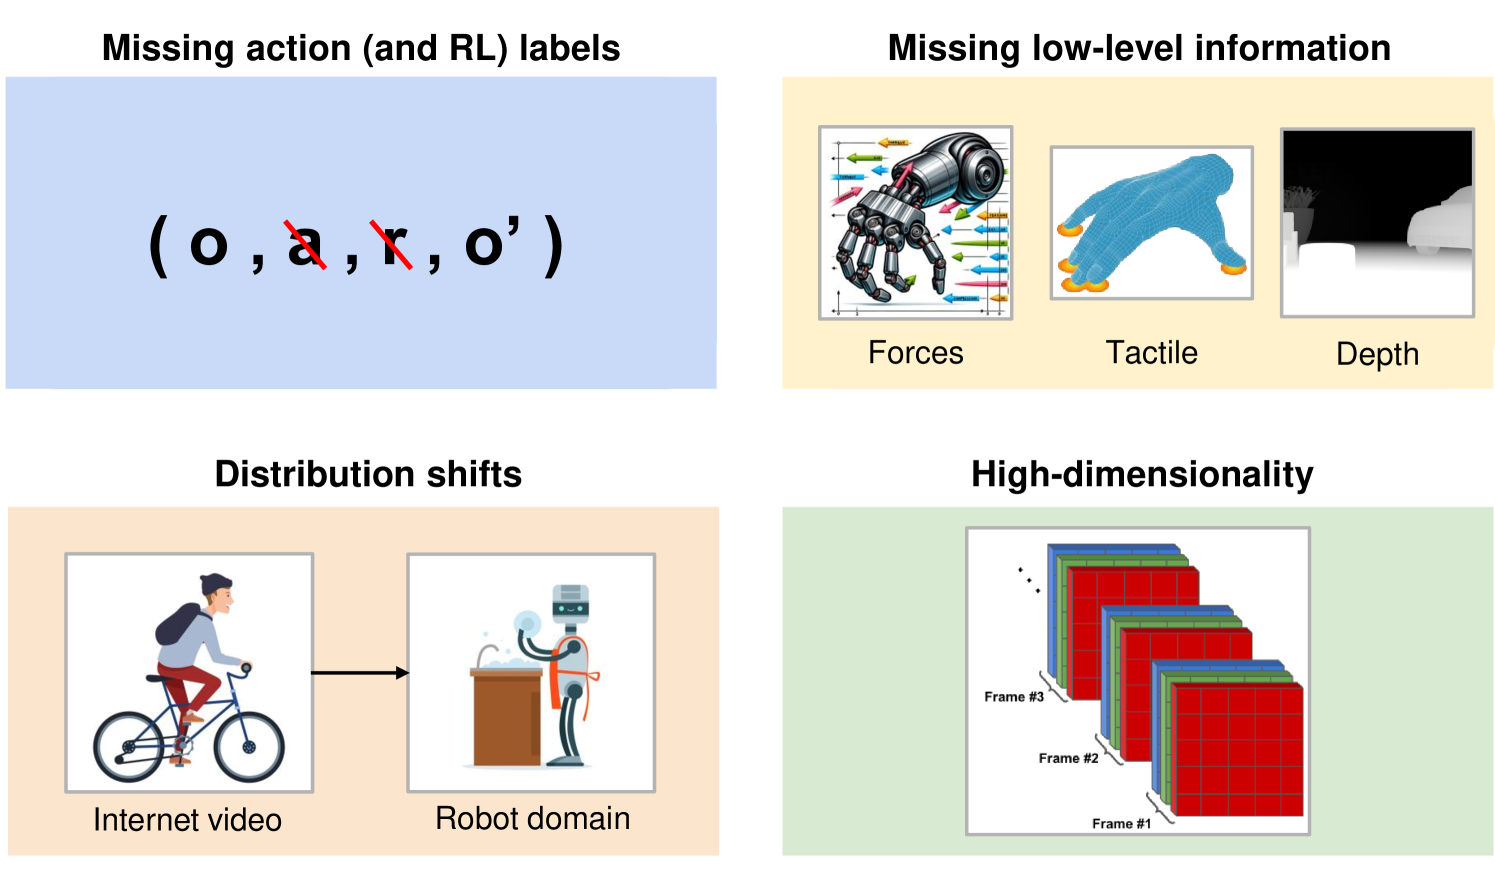
\includegraphics[width=1.0\linewidth]{./chapter4/media/KeyChallengesInLfV}
	\caption[Key Challenges in \acs{LfV}]{Key challenges in Learning from Videos. Image source: \cite{McCarthy_2025}.}
	\label{fig:KeyChallengesInLfV}
\end{figure}

\paragraph{Missing Action Labels}
One major limitation of raw video data is the absence of explicit action labels required by many \ac{IL} \cite{Brohan2022RT1RT} and offline \ac{RL} approaches \cite{Chebotar2023QTransformerSO}. While videos provide rich visual observations of behaviors, they typically do not contain the low-level control commands executed during the task. Retrospectively inferring robot actions from human videos is challenging, since human motions often cannot be directly mapped to the action space of a robotic system. Furthermore, videos usually lacks on \ac{RL} signals such as reward annotations, goal labels, or start-of- and end-of-episode boundaries \cite{McCarthy_2025}.


\paragraph{Missing Low-level Information}
Internet videos also lack on low-level sensory information. Skillful behaviors often depend on tactile feedback, force measurements, proprioceptive signals, or depth information, which are generally not observable in classical RGB videos. Although videos may capture high-level task structure and object interactions, they do not explicitly provide the fine-grained physical information necessary for learning accurate motor control and stable interaction with the environment \cite{McCarthy_2025}.


\paragraph{Distribution Shift}
Another challenge arises from the distribution shift between internet videos and the downstream robotics domain. Differences may occur in camera viewpoints, environments, embodiments, object appearances, and task distributions. The Human demonstrations in videos may contain behaviors that are inefficient, ambiguous, or irrelevant for robotic execution \cite{McCarthy_2025}.

In particular, \ac{LfV} must address the embodiment gap between humans and robots as they often differ significantly in their kinematics, morphology, and control capabilities. Furthermore, there exists a visual gap between the human actor performing the task in the video and the robotic embodiment that is expected to execute the task. As a result, transferring observed human motions directly to robot actions is highly non-trivial and requires models to learn embodiment-invariant task representations \cite{McCarthy_2025}.

Additionally, some important robotic tasks, such as specialized industrial manipulation tasks, may be difficult to learn because they are underrepresented in publicly available video datasets \cite{McCarthy_2025}.

\paragraph{High-dimensionality, Noise, and Redundancy}
Video data is inherently high-dimensional and often contains substantial amounts of irrelevant or redundant information. Background changes, camera motion, occlusions, and unrelated actions can make it difficult for models to identify task-relevant features, making it challenging to learn robust representations. Furthermore, the sheer volume of video data can lead to computational challenges in processing and learning from such large datasets \cite{bardes2024vjepa}.


\paragraph{Controllability, Stochasticity, and Partial Observability}
In unlabeled video data, it can be tricky for models to determine which changes in the environment are caused by the agent's actions and which originate from external factors or environmental noise \cite{Horan2021WhenIU}. This ambiguity makes it challenging to infer action information directly from video observations. Furthermore, real-world environments are frequently stochastic and only partially observable, meaning that important state information may be hidden from the camera viewpoint \cite{Babaeizadeh2017StochasticVV}. As a result, predicting future states or accurately modeling action consequences from video alone becomes a difficult problem.


\paragraph{Summary}
None of these challenges have yet been fully solved. In the following sections, we will discuss some possible ways to address these issues coming with internet video data. Nevertheless it seems likely that scaling — with the help of internet video data — can provide significant gains in robotic systems within the near future \cite{McCarthy_2025}.



% Existing LfV research has shown promising signs of life, and this is a field ripe for further progress. Of course,
% it is unclear whether scaling deep learning will take us all the way to general-purpose robots (Section 6.4), and
% there are other research directions that should be pursued in parallel (Section 2). Nevertheless, with sufficient
% effort and innovation, it seems likely that scaling—with the help of internet video data—can provide significant
% gains in the near-future



% **Missing Action Labels**

% - **video** lacks **information** critical to robotics, including action labels and low-level force and proprioceptive information

% **Missing Low-level Information**

% - For certain skillful behaviours, robots require low-level percepts such as tactile sensing, forces, proprioception, or depth sensing
%     - data not explicitly available in internet video.

% **Distribution-shift**

% - various distribution shifts between internet video and the robot domain.
% - shifts between an internet video dataset and the downstream robot domain.
%     - physical embodiments, camera viewpoints, tasks, and environments
% - Humans in videos may perform behaviours which are sub-optimal or irrelevant
% - useful tasks and behaviours may be underrepresented in internet video
% - **embodiments** from robots very **different from that of a human may prove more effective**

% **High-dimensionality, Noise, and Redundancy**

% - challenging to extract meaningful information and representations from video data
% - some important actions and tasks may be underrepresented in the video dataset
%     - e.g., specialized industrial tasks
%     - the robot may need to perform tasks not commonly performed by humans


% \subsection{Other Paths to Generalist Robots.}


% Goal: reduce the amount of robot videos

% - **Video provides foundational information:**
%     - Contains physics and dynamics information
%     - Shows human behaviors, tasks and actions relevant to robots
%     - High quantity and diversity
%     - Relatively untapped resource
%     - —>can be highly informative for general-purpose robots.
% use of diverse internet data has facilitated a transition from task-specific models to monolithic foundation models with more general capabilities


% \ac{LfV} will solve the data bottleneck by augmenting traditional robot data with large-scale internet video.















% \ac{IL} (IL) is a powerful approach for training agents to perform complex tasks by learning from demonstrations provided by an expert. The main advantage of IL is that it can leverage large datasets of human demonstrations, which are often easier to collect than reward signals. This allows IL to learn complex behaviors that are difficult to specify with a reward function, and can be more sample efficient than reinforcement learning, especially in high-dimensional state spaces.





% —> learning a KM from a video dataset and finetune it to the robot domain

% Different approaches to transfer the knowledge

% - **Generalisation and zero-shot transfer:**
% pretrained KM directly in the target setting, without further fine-tuning or adaptation
% - **Fine-tuning and Representation transfer:** 
% methods that train a model in the robot domain that is partially composed of parts of a pretrained KM
% - **Hierarchy: conditioning**
% involves using a pretrained KM to condition a new KM being trained in the target MDP




%  In-the-wild videos are particularly valuable for training robots to operate in diverse and unstructured environments, as they capture a wide range of scenarios, object appearances, lighting conditions, and background variations that the robot may encounter in real-world applications. However, learning from in-the-wild videos also introduces significant challenges, such as dealing with noisy data, occlusions, varying viewpoints, and the need for robust feature extraction to identify relevant information for task execution. Despite these challenges, leveraging in-the-wild videos can significantly enhance the generalization capabilities of robotic systems and enable them to perform effectively in real-world settings.
